\documentclass[tikz,border=10pt]{standalone}
\usepackage{tikz}
\usetikzlibrary{
    arrows.meta,
    positioning,
    quotes,
    shapes.geometric,
    backgrounds,
    fit,
    calc
}

\begin{document}
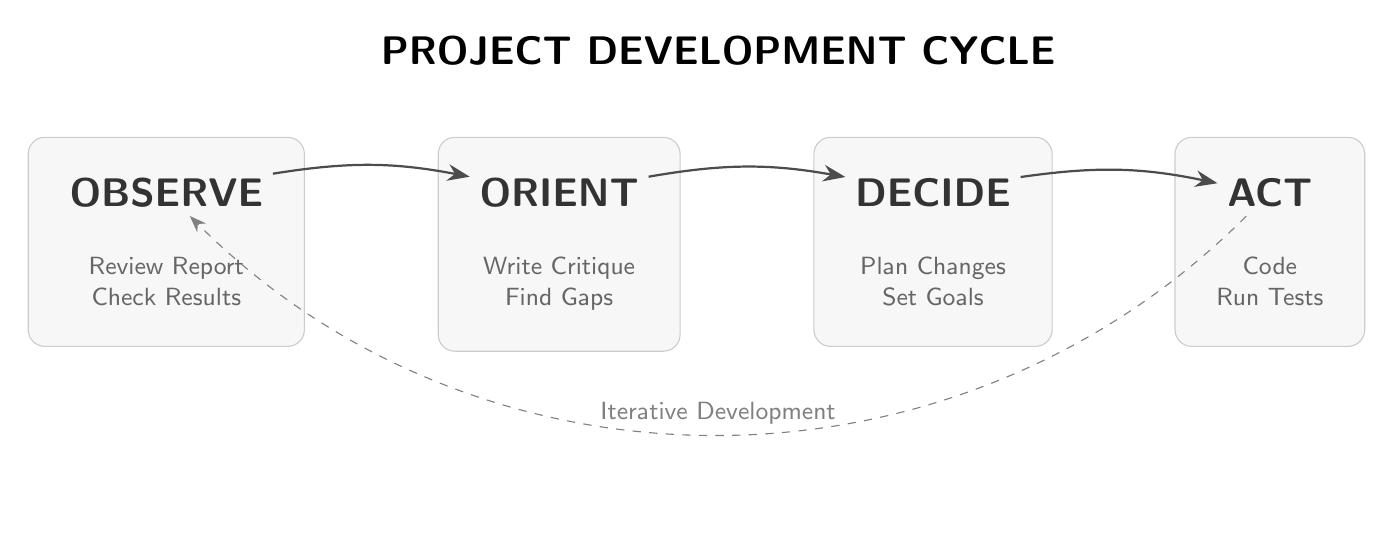
\begin{tikzpicture}[
    node distance=2.5cm,
    % Clean, modern styling
    phase/.style={
        font=\Large\sffamily\bfseries,
        text=black!80
    },
    detail/.style={
        font=\small\sffamily,
        text=black!60,
        align=center
    },
    mainflow/.style={
        -{Stealth[length=8pt]},
        thick,
        black!70
    },
    feedback/.style={
        -{Stealth[length=6pt]},
        dashed,
        black!50
    },
    container/.style={
        rounded corners=6pt,
        draw=black!20,
        fill=black!3,
        inner sep=0.4cm
    }
]
    % Calculate total width for centering
    \path (0,0) -- ++(12,0);
    
    % Main phases with more elegant spacing
    \node[phase] (observe) at (0,0) {OBSERVE};
    \node[phase, right=of observe] (orient) {ORIENT};
    \node[phase, right=of orient] (decide) {DECIDE};
    \node[phase, right=of decide] (act) {ACT};
    
    % Project-specific details
    \node[detail, below=0.4cm of observe] (obs-detail) {Review Report\\Check Results};
    \node[detail, below=0.4cm of orient] (ori-detail) {Write Critique\\Find Gaps};
    \node[detail, below=0.4cm of decide] (dec-detail) {Plan Changes\\Set Goals};
    \node[detail, below=0.4cm of act] (act-detail) {Code\\Run Tests};
    
    % Subtle containers
    \begin{scope}[on background layer]
        \node[container,fit=(observe)(obs-detail)] {};
        \node[container,fit=(orient)(ori-detail)] {};
        \node[container,fit=(decide)(dec-detail)] {};
        \node[container,fit=(act)(act-detail)] {};
    \end{scope}
    
    % Flowing main arrows
    \draw[mainflow] (observe) to[bend left=10] (orient);
    \draw[mainflow] (orient) to[bend left=10] (decide);
    \draw[mainflow] (decide) to[bend left=10] (act);
    
    % Elegant feedback loop with project focus
    \draw[feedback] (act) to[bend left=45] node[above, font=\small\sffamily] {Iterative Development} (observe);
    
    % Centered title with breathing room
    \node[font=\Large\sffamily\bfseries, above=1.5cm] at ($(observe)!0.5!(act)$) {PROJECT DEVELOPMENT CYCLE};
\end{tikzpicture}
\end{document} 